\chapter{基础知识}

本章节介绍了本文的技术路线所使用到的一些基础知识概念和密码学工具,包括同态加密的基本概念、全同态加密方案 CKKS 及其功能、格密码学库 Lattigo、椭圆曲线签名算法 ECDSA 以及 Golang 等。

\section{同态加密综述}

同态加密的概念源于 Rivest 等人于 1978 年提出的隐私同态(Privacy Homomorphic)概念\cite{rivest1978data},用户将个人敏感数据加密后存储在一个不可信的服务器中,允许服务器在没有私钥,不了解明文的情况下,完成对密文的处理任务,并给出正确的查询应答。\cite{FHEResearch}

依据各加密方案支持的同态运算种类和运算次数等,目前学界主要将同态加密算法分为以下数种:
\begin{itemize}
    \item 部分同态加密(Partial HE):PHE 指一种支持对密文进行无限次单一类型运算的加密方案,例如仅支持加法或乘法中的一种运算。PHE 大多都出现在全同态加密出现前,代表性方案有 Paillier 和 RSA 等,前者允许对密文进行无限次加法运算,后者允许对密文进行无限次乘法运算。
    \item 类同态加密(Somewhat HE):SWHE 支持对密文数据进行有限数量的加法和乘法运算,随着运算次数的增加,密文数据的噪声也会随之增加,最终导致解密失败。大多数 FHE 方案都由 SWHE 方案演化而来。
    \item 全同态加密(Fully HE):和上面两种不同,FHE 允许对密文进行任意次数的多种运算。FHE 方案的出现,使得密文数据的运算次数不再受限制,从而使得密文数据的计算能力大大提升。
\end{itemize}

在第一个全同态加密方案被提出之前,就有许多传统加密方案就具有部分同态性,如 RSA 和 ElGamal 方案具有乘法同态性\cite{rivest1978method,elgamal1985public},而 Paillier 方案具有加法同态性\cite{paillier1999public}。2009 年,斯坦福大学的博士研究生 Craig Gentry 在该领域做出了重大突破,在他的博士毕业论文中,基于理想格提出了第一个全同态加密解决方案\cite{homenc}。Craig 的成果标志着第一代全同态加密方案的诞生,也标志着同态加密的研究进入了一个新的阶段。

2011 年至 2012 年间,Brakerski 等人首次利用 LWE 问题及 R-LWE 问题的困难假设,构造了第二代全同态加密方案\cite{cryptoeprint:2011/344,cryptoeprint:2011/277,cryptoeprint:2012/144}。这些方案分别被命名为 BGV 和 BFV。在这之后的 2013 年,Gentry 和 Sahai 等人利用近似特征向量,构建了 GSW(Gentry-Sahai-Waters) 方案,标志着第三代方案的产生。而后学界又基于 GSW 方案,提出了其他两个加密系统:FHEW\cite{fhew} 和 TFHE\cite{TFHE},这些方案具有良好的加解密性能和自举性能。然而,上述算法均只支持对整数进行运算。2016 年,第一个允许对浮点数进行同态运算的加密方案 CKKS 被提出\cite{cryptoeprint:2016/421}。CKKS 方案的出现,使得同态加密的应用范围得到了极大的扩展。

\section{全同态加密方案 CKKS}

\subsection{R-LWE问题}

LWE(Learning with errors) 问题是一个机器学习领域中的怀疑难解问题,由 Regev 等人提出\cite{10.1145/1568318.1568324},该问题的困难性亦被应用于公钥密码学领域。简单地说,LWE 问题是一种通过向秘密值向量引入噪声来隐藏秘密值向量的方法。

% TODO: 考虑插入学术定义

R-LWE (Ring-LWE)问题由 LWE 问题衍生,将 LWE 问题拓展至多项式环上。该问题被认为是抗量子计算的。基于 R-LWE 问题已有许多应用被提出,如密钥交换算法\cite{cryptoeprint:2012/688}和数字签名算法\cite{cryptoeprint:2011/537}。

% TODO: 也考虑插入学术定义

\subsection{CKKS 方案综述}

CKKS(Cheon-Kim-Kim-Song) 方案,又称为 HEAAN(Homomorphic Encryption for Arithmetic of Approximate Numbers),是一种允许对全体复数向量域 $\mathbb{C}^{N/2}$ 进行同态运算的全同态加密方案。其安全性来源于 R-LWE 问题的决策版本。该方案的主要特点在于以一定误差为代价,允许对复数值向量进行计算。这一关键特性意味着其突破了先前提出的同态加密方案只能对整数进行运算的限制,对于许多实际应用来说非常重要。目前 CKKS 已经集成至诸多流行的密码学库,包括 SEAL、OpenFHE 和 Lattigo 等\cite{sealcrypto,OpenFHE,Mouchet2020LattigoAM},并受到来自开源社区的优化和维护。

与以往同态加密方案将噪声空间和明文空间分开的设计不同,CKKS 方案将噪声视为明文的一部分,而噪声一方面来源于基于 R-LWE 的加密方案中为保证安全性而人为加入的误差,另一方面也来源于近似计算中的舍入误差。密文解密后不能将明文中的噪声去除,只能以预定的精度 $\Delta$ 输出明文的近似值。\cite{CKKS_optimize}

CKKS 方案由首尔大学的 Cheon 等人在 ASIACRYPT17 上首次提出\cite{cryptoeprint:2016/421},此时其属于层级全同态加密,即只支持在预定层级内进行密文之间的同态乘法,当层级降低至 0 后,密文之间的同态乘法将不再可用。随后在 2018 年 Cheon 等人提出了 CKKS 方案的自举方法\cite{cryptoeprint:2018/153},允许刷新密文的层级。该成果将该方案拓展至全同态加密。同一年晚些时候,Cheon 等人提出了 CKKS 方案的余数系统变种,极大地提升了原方案的性能。\cite{cryptoeprint:2018/931}此外,亦有实验性的使用多项式近似对两个密文进行比较的算法被提出\cite{cryptoeprint:2019/417,cryptoeprint:2019/1234,cryptoeprint:2020/834}。

CKKS 方案包含以下的核心函数和算法:

\begin{itemize}
    \item $KeyGen(\lambda) \rightarrow sk, pk, evk$:密钥生成算法,输入安全参数 $\lambda$,输出公钥 $pk$ 和私钥 $sk$,以及评估密钥 $evk$。
    \item $Ecd(z; \Delta) \rightarrow m$:对消息进行编码的算法,输入一个复向量 $z \in \mathbb{Z}^{N/2}$,输出编码后的明文 $m \in R_q = \mathbb{Z}_q[X]/(X^N+1)$;其中 $m$ 为该明文编码后对应的多项式,$\Delta$ 为编码的精度,$N$ 为该向量的最大长度。
    \item $Dcd(m; \Delta) \rightarrow z$ :将上述编码后的明文解码为复向量的算法,输入编码后的明文 $m$,输出解码后的复向量 $z$。
    \item $Enc_{pk}(m) \rightarrow ct$ :使用公钥 $pk$ 对明文 $m$ 进行加密,输出密文 $ct = (c_0(X),c_1(X)) \in R_Q^2, R_Q = Z_Q[X]/(X^n + 1)$。
    \item $Dec_{sk}(ct) \rightarrow m'$ :使用私钥 $sk$ 对密文 $ct$ 进行解密,输出明文 $m'$
    \item $Add(ct_1, ct_2)$ :对密文进行加法运算的算法,输入两个密文 $ct_1$ 和 $ct_2$,输出加法运算后的密文 $ct_{add} = ct_1 + ct_2 = Enc_{pk}(m_1 + m_2)$。
    \item $Mult_{evk}(ct_1, ct_2) = ct_1 \bullet ct_2$:对密文进行乘法运算,输入两个密文 $ct_1$ 和 $ct_2$,输出乘法运算后的密文 $ct_{mult} = ct_1 \bullet ct_2 = Enc_{pk}(m_1 \bullet m_2)$。
    \item $MultByConst(ct, const) = ct'$:对密文乘上一个明文常数。在 Lattigo 中该方法无需评估密钥 $evk$ 即可进行。\cite{lattigoRepo}
\end{itemize}

此外也包括以下的辅助函数:

\begin{itemize}
    \item $Rescale(ct, r) \rightarrow ct'$:即密文的重缩放过程。输入密文 $ct$ 和重缩放的精度 $r$,输出重缩放后的密文 $ct'$,其中 $ct'$ 具有更小的模数 $q' = q \bullet r^{-1}$。重缩放操作作为一种有效的密文噪声控制手段,在 CKKS 方案中起到了关键作用,有效地将同态乘法带来的噪声增长速率从指数级控制到线性级。
    \item $Rotate_{evk}(ct, k) \rightarrow ct'$:密文的旋转操作。输入密文 $ct$ 和旋转的位数 $k$,输出旋转后的密文 $ct'$。
\end{itemize}

得益于 R-LWE 问题允许对密文的密钥进行转换\cite{brakerski2014leveled},CKKS 加密方案亦适用于以下重加密方法:

\begin{itemize}
    \item $GenSwk(sk_1, sk_2) \rightarrow swk$:以私钥 $sk_1$ 和 $sk_2$ 为输入,输出用于进行密钥转换的重加密密钥 $swk$。
    \item $SwitchKey_{swk}(ct_{pk_1}) \rightarrow ct_{pk_2}$:该函数将密文 $ct_{pk_1}$ 转换为 $pk_2$ 对应的密文 $ct_{pk_2}$。
\end{itemize}

下图\cite{ckksIntroduct} \ref*{Fig:CKKS}描述了 CKKS 方案的工作生命周期:

\begin{figure}[ht]
    \centering
    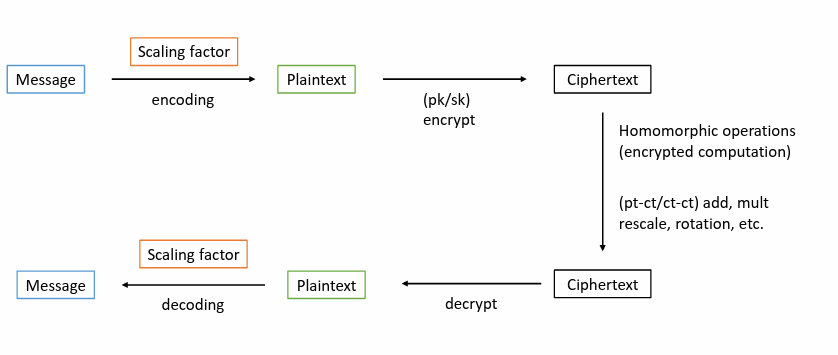
\includegraphics[width=0.8\linewidth]{./Figures/CKKS_Diagram.png}
    \caption{CKKS 方案工作示意图}\label{Fig:CKKS}
\end{figure}

\section{数字签名算法}

\subsection{数字签名算法综述}

数字签名是一种使用了公钥密码学的技术,于 1976 年被首次提出\cite{1055638}。其原理为对于某一信息,该算法可以使用私钥生成该信息的一个签名,并且可以被公钥验证。若验证不通过,则认为该信息被受到修改不是原信息;反之则可以确认该签名是由私钥持有者生成的,即该信息是由私钥持有者发送的。数字签名的应用领域包括防止消息纂改,以及验证某一消息是否真实地由某人发出。

\subsection{ECDSA}

椭圆曲线数字签名算法(Elliptic Curve Digital Signature Algorithm, ECDSA)是一种基于椭圆曲线密码学的数字签名算法,由 DSA 签名算法与椭圆曲线密码体制结合而成,并逐渐成为 ANSI\footnote{American National Standards Institute,美国国家标准学会}、IEEE\footnote{Institute of Electrical and Electronics Engineers,电气电子工程师学会}、ISO\footnote{International Organization for Standardization,国际标准化组织} 和 NIST\footnote{National Institute of Standards and Technology,美国国家标准技术研究所} 标准\cite{ecdsa_blockchain}。 

ECDSA 包含以下方法:

\begin{itemize}
    \item $KeyGen(\lambda) \rightarrow sk, pk$:输入安全参数 $\lambda$\footnote{通常为某一椭圆曲线},输出一对随机生成的私钥 $sk$ 和公钥 $pk$。
    \item $Sign(m, sk) \rightarrow sig$:使用私钥 $sk$ 对消息 $m$ 进行签名,输出签名 $sig$。
    \item $Verify(m, pk, sig) \rightarrow bool$:使用公钥 $pk$ 对签名 $sig$ 进行验证,输出验证结果 $bool$。
\end{itemize}

\section{Lattigo}

Lattigo 是一个 Golang 密码学库,实现了多个基于 R-LWE 问题的全同态加密方案,以及数个安全多方计算协议。\cite{Mouchet2020LattigoAM,lattigoRepo}该密码学库具有以下的特点:

\begin{itemize}
    \item 对目前学界流行的数个全同态加密方案,包括 BFV、BGV 和 CKKS 以及它们对应的多方计算版本,其中 CKKS 也包括了它的一个变种\cite{cryptoeprint:2018/952}。此外该库也支持 CKKS 的自举操作,使得该方案可以进行全同态加密。
    \item 使用 Golang 编写。该语言及其工具链本身的特点使得其十分适合进行网络编程和异步编程,同时也拥有着与 C/C++ 库相当的性能,甚至在某些情况下更优。此外,Go 工具链也有着较为完备的集成测试框架。
    \item 良好的跨平台特性。该密码学库支持所有 Golang 本身支持的平台,也包括了浏览器所使用的,和具体平台无关的 Web Assembly 代码。
\end{itemize}

\section{SQLite3}

SQLite3 是一个轻量级的开源的关系数据库,其源代码被释放在公有领域\cite{sqlite3}。和其他数据库管理系统不同,SQLite 最大的特点没有单独的服务器进程,只作为一个程式库在单个数据库文件中进行操作。这一特性使得 SQLite 不需要进行额外配置,直接嵌入到应用程序中运行。SQLite3 所使用的数据库文件格式也是开放且稳定的。许多流行的语言,如 Python、Rust,以及本文所使用的 Golang,都有 SQLite3 的第三方库,在静态编译的情况下,程序本身并不需要系统安装 SQLite3 运行时库。

SQLite3 的主要特性如下:\cite{sqlite3_2}

\begin{itemize}
    \item 独立性:SQLite 是一个独立的系统,除了 C 标准库以外几乎没有其他任何依赖关系,因此几乎能够在所有的操作系统上运行
    \item 零配置:SQLite 不需要进行额外的配置,也不需要服务器进程,所有的数据都存储在一个单独的文件中。SQLite 可以作为动态或静态链接库嵌入应用程序,而且大多数语言都有对应的第三方库。
    \item 事务性:和其他数据库一样,SQLite 也支持事务,而且支持 ACID 属性。对SQLite嵌入式数据库来说,单个事务中的所有更改要么完全触发,要么根本不发生。
\end{itemize}

%\section{REST API}
% 视情况考虑是否保留
%REST(Representational State Transfer),即表现层状态转换,是一种网络软件架构风格。它具有以下的特点:

%\begin{itemize}
%    \item 客户端-服务端架构:
%    \item 统一的接口
%    \item 无状态的通信
%\end{itemize}

\section{本章小结}

本章首先介绍了同态加密和全同态加密,及其发展历程。然后,本章重点介绍了本文所使用的全同态加密方案 CKKS,包括其基于的困难问题,CKKS 方案的特点,以及该加密方案包含的主要函数等。本章也对椭圆曲线签名算法等涉及到的其他密码学工具,进行了简要的介绍。另外本章也简要介绍了后文中会用到的软件工具,包括全同态加密密码学库 Lattigo 和数据库引擎 SQLite 3,为后续的实现进行准备。本章内容是后文的基础,后续对交易方案的构建都在本章基础之上完成。
